\DiaryEntry{Single-Source Shortest Paths}{2020-04-02}{Algorithms}

\subsection{Introduction}

We are given a weighted, directed graph $G=(V,E)$ with a weight function $w: E \rightarrow \mR$ mapping edges to real-valued weights. A path $p$ is a sequence of edges, $p=\langle v_0,v_,\cdots,v_n \rangle$; its \emph{weight} $w(p)$ is given by the sum of its edges

\bee
w(p) = \sum_{i=1}^n w(v_{i-1},v_i)
\eee

The \emph{shortest-path weight} $\delta(u,v)$ from vertex $u$ to vertex $v$ is defined as

\bee
\delta(u,v) = \begin{cases} \min_p w(p): u \rightarrow v \, & \text{if there is a path from u to v} \\ \infty \, & \text{otherwise} \end{cases}
\eee

A \emph{shortest path} from $u$ to $v$ is then any path from $u$ to $v$ with weight $w(p) = \delta(p)$. There can be more than one shortest path between $u$ and $v$.

In this entry, we focus on \emph{single-source shortest paths problems}; i.e. we are given one source egde $s \in V$ and determine shortest paths to all vertices $v \in V$. 

The followig theorem helps in  with finding shortest paths.

\begin{theorem}
Given a weighted graph $G=(V,E)$ with weight function $w: E \rightarrow \mR$, let $p=\langle v_0,v_,\cdots,v_n \rangle$; be a shortest path from vertex $v_0$ to vertex $v_n$, and, for any $i$ and $j$ such that $0 \leq i \leq j \leq n$, let $p_{ij} = \langle v_i,v_,\cdots,v_j \rangle$ be the subpath of $p$ from vertex $v_i$ to vertex $v_j$. Then, $p_{ij}$ is a shortest path from $i$ to $j$. 
\end{theorem}


\paragraph{Example.} We consider the following weighted graph as example.


\begin{figure}[H]
\centering
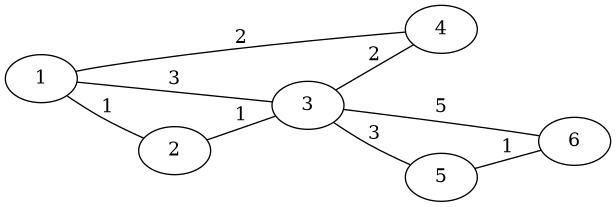
\includegraphics[scale=0.5]{images/sssp_1.png}
\end{figure}


If we choose the source vertex $s=1$ and run a single-source shortest path algorithm (Bellman-Ford), we obtain the following result: The algorithm returns a tree (via a predecessor graph) which is shown in red in the Figure below.


\begin{figure}[H]
\centering
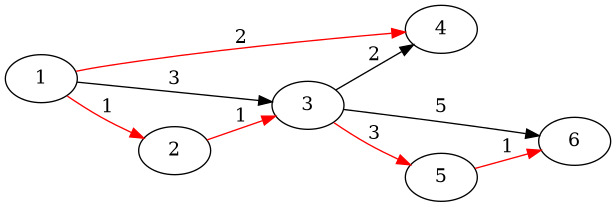
\includegraphics[scale=0.5]{images/sssp_2.png}
\end{figure}

In addition, the algorithm provides the distance between the source and each vertex. This is shown in the Table below.

\begin{tabular}{c|c}
  Vertex & Distance \\ \hline
  1 & 0 \\
  2 & 1 \\
  3 & 2 \\
  4 & 2 \\
  5 & 5 \\
  6 & 6
\end{tabular}



%%% Local Variables:
%%% mode: latex
%%% TeX-master: "journal"
%%% End:
